\documentclass[t]{beamer}

\usepackage{biblatex}
\usepackage{algorithm}
\usepackage{src/templates/algorithmicx/algpseudocode}

\setbeamerfont{footnote}{size=\tiny}

\input{header-presentation}
\title[FPGA for BING!]{A Reconfigurable Fabric for Accelerating Large-Scale Datacenter Services}
\author[bobzhou@bu.edu]{Reviewed by Boyou Zhou}
\date[\today]{\today}

\begin{document}
\maketitle

\section*{FPGA for BING!}

\section{Intro: Why FPGA?}

\begin{frame}{What is ASIC, FPGA and GPP?}
    \begin{block}{ASIC}
        \begin{itemize}
            \item Application Specific Integrated Circuit
            \item Performance: Best, Cost: Highest, Time to Market: Slowest
        \end{itemize}
    \end{block}
    \begin{block}{FPGA}
        \begin{itemize}
            \item Field Programmable Gate Array
            \item Performance: Good, Cost: Normal, Time to Market: Normal 
        \end{itemize}
    \end{block}
    \begin{block}{GPP}
       \begin{itemize}
            \item General Purpose Processor
            \item Performance: Worst, Cost: Lowest, Time to Market: Fastest
       \end{itemize} 
    \end{block}
\end{frame}

\begin{frame}{Time to Market Comparison Between FPGA, and ASIC}
    \begin{figure}
        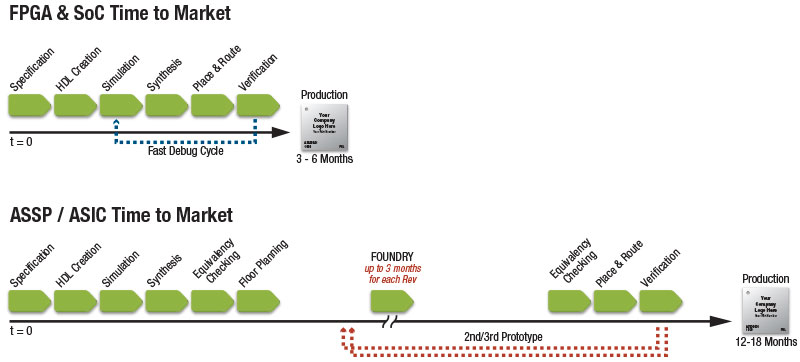
\includegraphics[width=4in]{img/design-time-comparison.png}
        \caption{Time to Market comparison\footcite{http://www.rtcmagazine.com/articles/view/102721}}
        \label{fig:time-to-market}
    \end{figure}
\end{frame}

\begin{frame}{Cost Comparison Between FPGA, and ASIC}
    \begin{figure}
        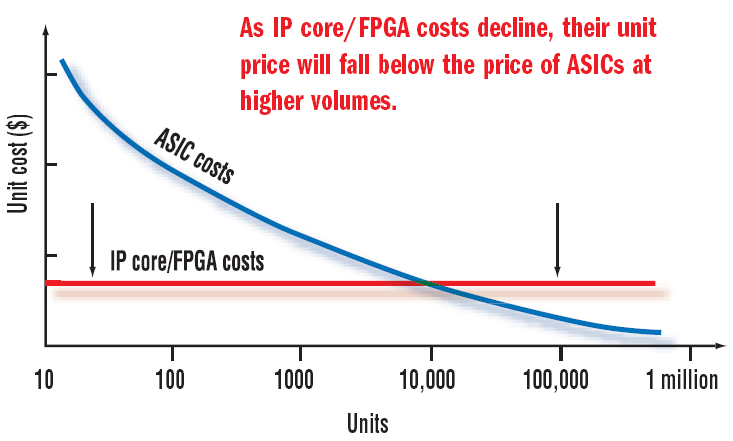
\includegraphics[width=2in]{img/FPGA-cost.png}~
        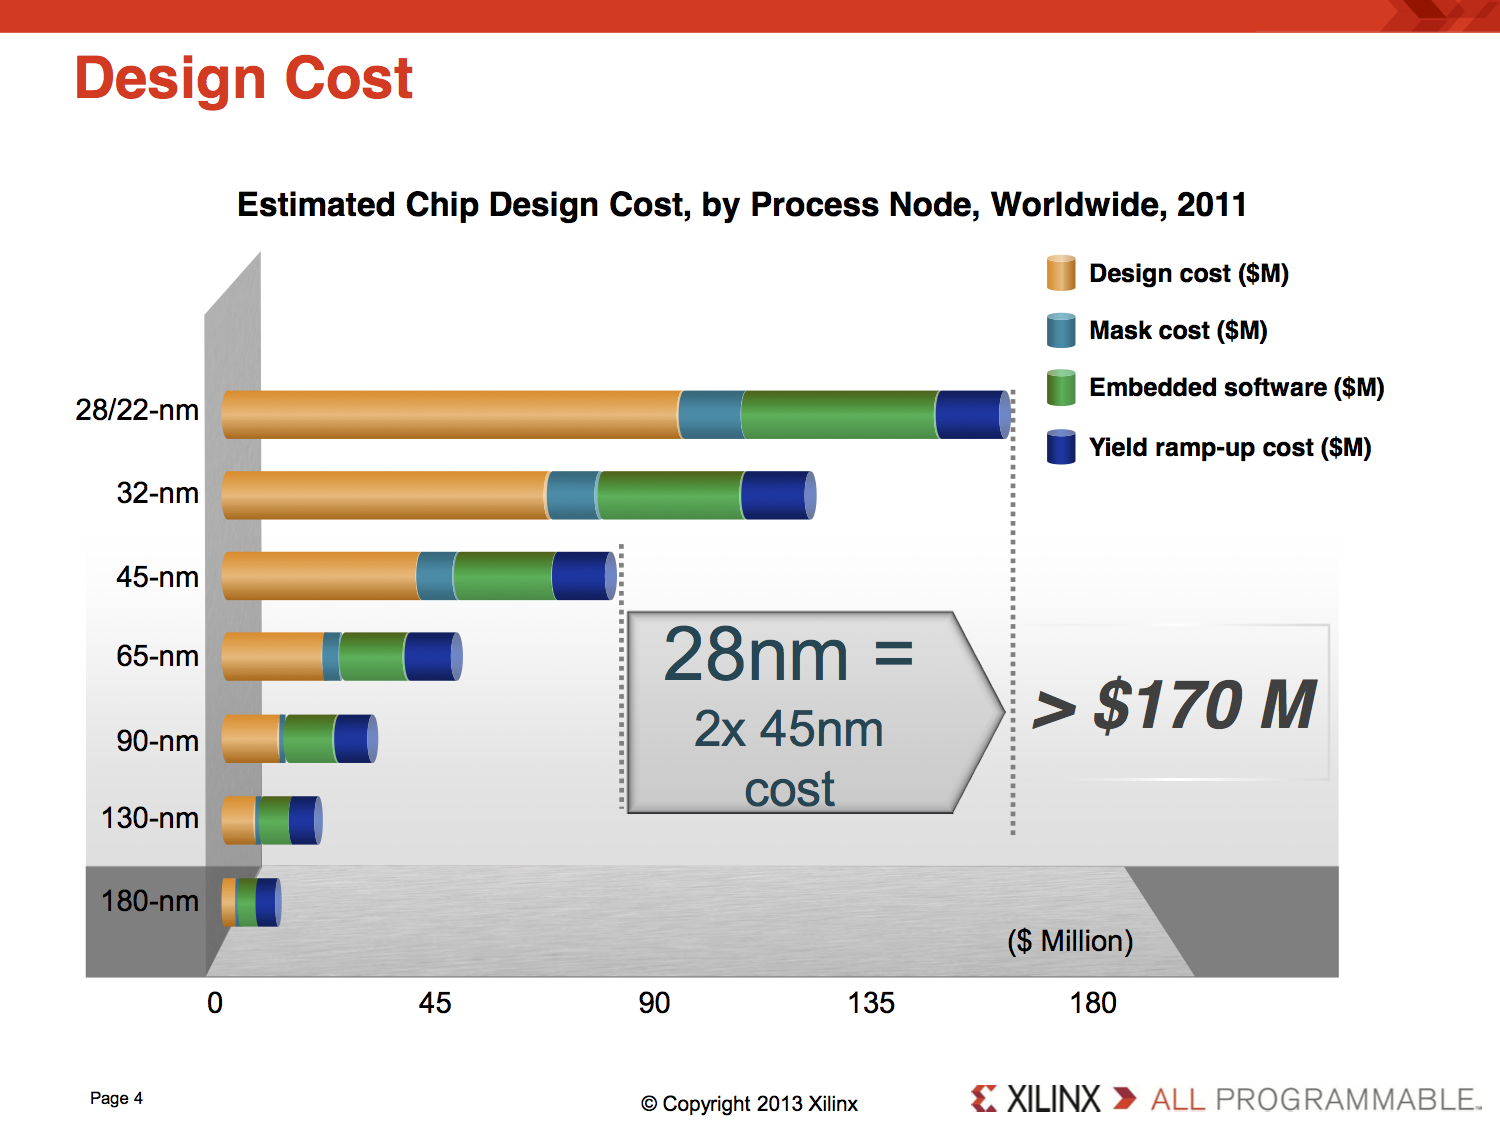
\includegraphics[width=2in]{img/ASIC-cost.png}
        \caption{FPGA cost\footcite{http://electronicdesign.com/files/29/12966/figure_01.gif}
                 ASIC cost\footcite{http://electroiq.com/blog/2014/02/semi-iss-scaling-innovation/}}
        \label{fig:cost-comparison}
    \end{figure}
\end{frame}

\begin{frame}{Performance Comparison Between GPP, FPGA, and ASIC}
    \begin{figure}
        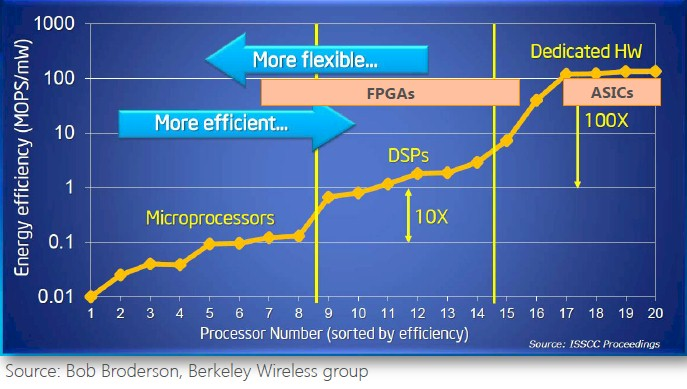
\includegraphics[width=4in]{img/microsoft-fpga-vs-cpu-vs-asic.png}
        \caption{FPGA, FPGA, and ASIC comparison from Microsoft\footcite{http://www.theplatform.net/2015/03/30/why-intel-might-buy-fpga-maker-altera}}
        \label{fig:performance-comparison}
    \end{figure}
\end{frame}

\section{Main Work: Use FPGA for Bing}
\begin{frame}{Resolved Problems}
    \begin{block}{Resolved Problems}
        \begin{itemize}
            \item {\tt{Homogeneity Design}} \\
            Homogeneity design reduces management issues and provide consistent platform to
            rely on.
            \item {\tt{Processing Speed}} \\
            Datacenter requests for extreme speed, which CPUs do not provide. 
        \end{itemize}
    \end{block}
\end{frame}

\begin{frame}{Solution and Evaluation}
    \begin{block}{Solution: reconfigurable Fabric, catapult Fabric}
        \begin{itemize}
            \item Each server has its own FPGAs and local DRAMs. 
            \item FPGAs are wired to each other in 6x8 two-dimensional torus, and provide hardware
            solution to desired functionality.
            \item Documents are processed through 8 pipelines of FPGAs.
        \end{itemize}
    \end{block}

    \begin{block}{Evaluation: search requests from Bing}
        \begin{itemize}
            \item 2x throughput compared to software approach in the number of docs ranked per
            second per server
        \end{itemize}
    \end{block}
\end{frame}

\begin{frame}{What is on board?}
    \begin{itemize}
        \item {\tt{8 GB of DRAM consists of two dual-rank DDR3-1600 SO-DIMMs}}
        \item {\tt{High-end Altera Stratix V D5 FPGA}}
        \item {\tt{A programmable oscillator}}
        \item {\tt{32 MB of Quad SPI flash to hold FPGA configurations}}
    \end{itemize}
\end{frame}

\begin{frame}{Hardware Deployment}
    \begin{figure}
        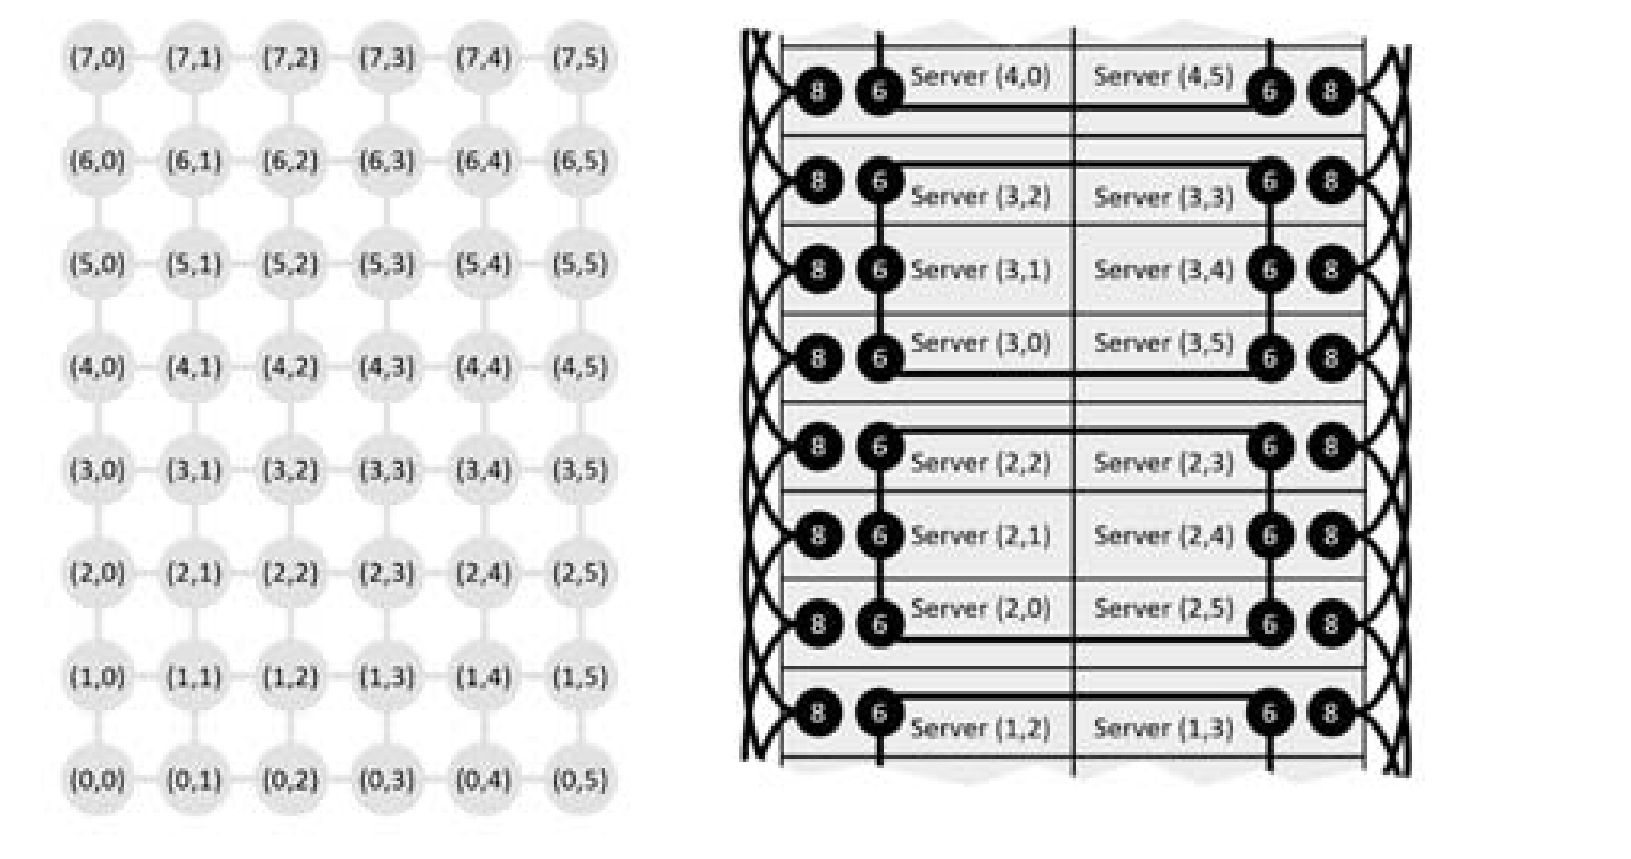
\includegraphics[width=4in]{img/torus-network.png}
        \caption{Logic mapping of the torus network}
        \label{fig:torus-network}
    \end{figure}
\end{frame}

\begin{frame}{Software Implementation}
    \begin{figure}
        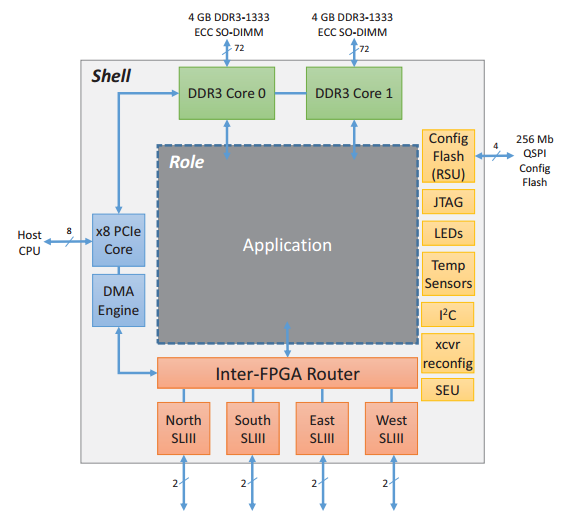
\includegraphics[width=2.5in]{img/shell-architecture.png}
        \caption{Shell Architecture}
        \label{fig:shell-architecture}
    \end{figure}
\end{frame}

\begin{frame}{Application Analysis: High Level Description}
    \begin{itemize}
        \item Data Arrives at Front-End cache service
        \item If a reuest is missed, it is routed to a top-level aggregator (TLA).
        \item TLA selects a machine.
        \item TLA sends the query to the target machine.
        \item The target machine performs a ranking service.
    \end{itemize}
\end{frame}

\begin{frame}{Application Analysis: Ranking service}
    \begin{itemize}
        \item Query words are the keywords and the document is the file to process.
        \item {\tt{Software:}} 
            \begin{itemize}
                \item Retrieve both query and document to a metastream
                \item Generate hit vectors
                \item Software generated features, such as numbers of hits.
            \end{itemize}
        \item {\tt{FPGA:}} 
            \begin{itemize}
                \item Synthetic features are computed, such as Free-Form Expressions.
                \item Features are sent to machine leant model to generate a score.
            \end{itemize}
    \end{itemize}
\end{frame}

\begin{frame}{Pipeline Stages}
    \begin{figure}
        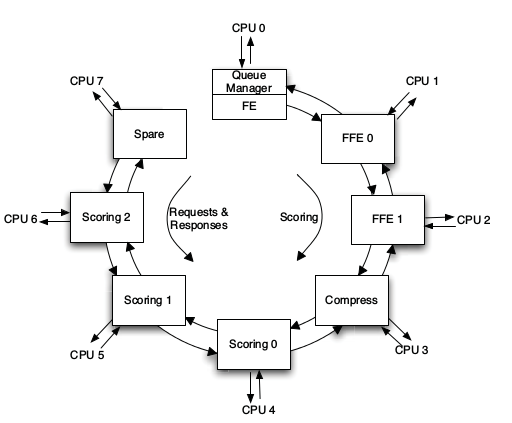
\includegraphics[width=2.5in]{img/fpga-pipeline.png}
        \caption{8 FPGAs in pipeline}
    \end{figure}
\end{frame}

\begin{frame}{Pipeline Stages}
    \begin{itemize}
        \item Feature Extraction
        \item 2 $\times$ Free-Form Expression
        \item Compression
        \item 3 $\times$ Machine-learned Score Models
        \item Rotate the ring if there is a system failure
    \end{itemize}
\end{frame}

\begin{frame}{Model Reload and Queue Manager}
    \begin{itemize}
        \item Models: Different sets of features and free forms. Model reloading takes about 250 $\mu
        s$, while reconfiguration takes about miliseconds or seconds.
        \item Queue Manager: Query and documents are stored in queues in the DRAM. QM switch queues when
        data are processed.
    \end{itemize}
\end{frame}

\section{Evaluation}

\begin{frame}{Troughput Comparison}
    \begin{figure}
        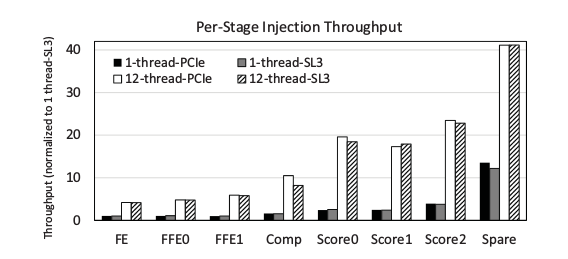
\includegraphics[width=4in]{img/throughput-comparison.png}
        \caption{Each Stage Throughput Comparison}
    \end{figure}
\end{frame}

\begin{frame}{Latency Comparison}
    \begin{figure}
        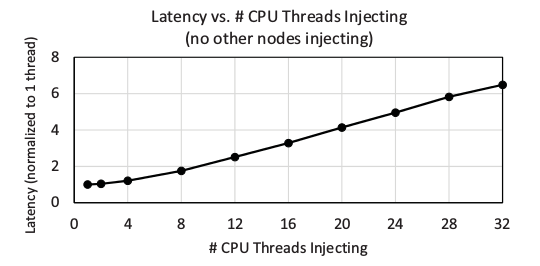
\includegraphics[width=4in]{img/latency-cpu-fe.png}
        \caption{Latency with different number of threads injection in FE stage}
    \end{figure}
\end{frame}

\begin{frame}{Document Injection Rate}
    \begin{figure}
        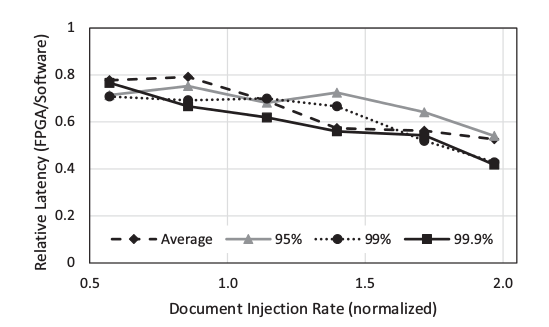
\includegraphics[width=4in]{img/document-injection-rate.png}
        \caption{Document Injection Rate}
    \end{figure}
\end{frame}

\begin{frame}{Throughput increase}
    \begin{figure}
        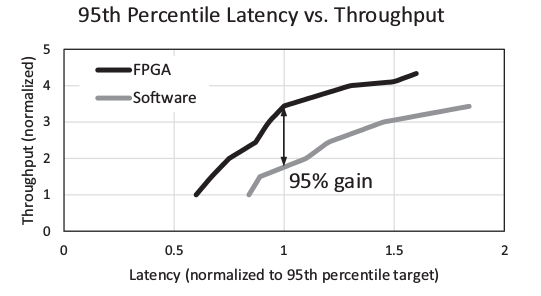
\includegraphics[width=4in]{img/throughput-increase.png}
        \caption{Throughput increase}
    \end{figure}
\end{frame}

\begin{frame}{Node Latency Injection}
    \begin{figure}
        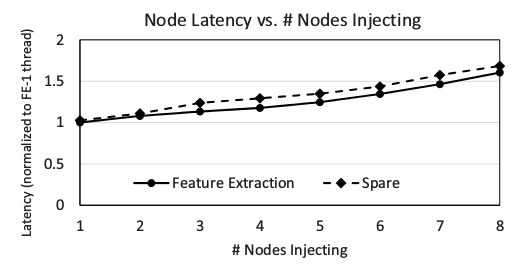
\includegraphics[width=4in]{img/node-latency-injection.png}
        \caption{Node Latency Injection}
    \end{figure}
\end{frame}

\begin{frame}{CPU Throughput Threads}
    \begin{figure}
        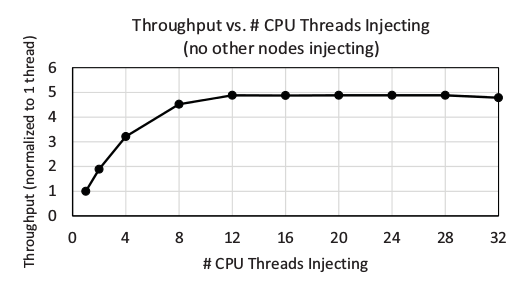
\includegraphics[width=4in]{img/throughput-cpu-thread.png}
        \caption{Throughput CPU Threads}
    \end{figure}
\end{frame}


\end{document}
